\documentclass{beamer}

\usepackage{subcaption}
\usepackage[backend=bibtex]{biblatex}
\addbibresource{bib/main.bib}

\newcommand\fixme[2][FIXME]{\textcolor{red}{\textbf{#1:} #2}}
\usepackage[labelsep=space]{caption}
\usepackage[ruled, vlined, linesnumbered]{algorithm2e}

\SetKwInput{KwInput}{Input}
\SetKwInput{KwOutput}{Output}

\usepackage{amsmath}
\DeclareMathOperator*{\argmax}{arg\,max}

\usetheme[subsectionpage=progressbar, progressbar=frametitle]{metropolis}
\setbeamerfont{footnote}{size=\tiny}

\definecolor{turquoise}{RGB}{64,224,208}
\definecolor{turqbrown}{RGB}{92,80,60}
\setbeamercolor{progress bar}{fg=turquoise}
\setbeamercolor{normal text}{fg=turqbrown}
\title{Research Update}
\author{W. Cannon Lewis II}

\date{May 19, 2021}

\begin{document}
\begin{frame}
  \titlepage
\end{frame}

\section{Motivation}

\begin{frame}{Industrial Robotics}
  Industrial robots are heavy, dangerous, and expensive

  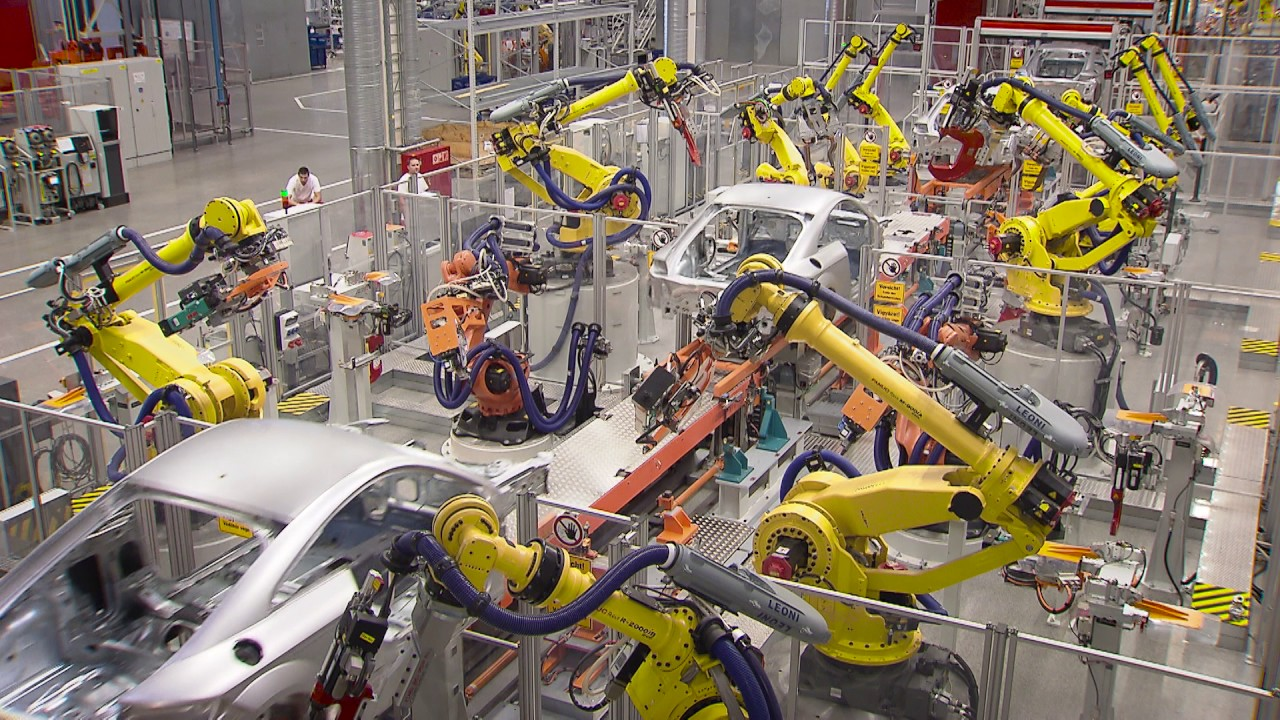
\includegraphics[keepaspectratio,width=\textwidth]{assets/factory_robots}
\end{frame}

\begin{frame}{Hardware Solving Software}
  Why are industrial robots heavy, dangerous, and expensive? 
  \begin{itemize}
    \item Hardware robustness
    \item Quasistatic assumptions
    \item Correction for noise by applying large torques
  \end{itemize}
\end{frame}

\begin{frame}{Beyond Industrial Robots}
  Agile robots like Spot are still expensive and require extensive human guidance.

  \begin{center}
    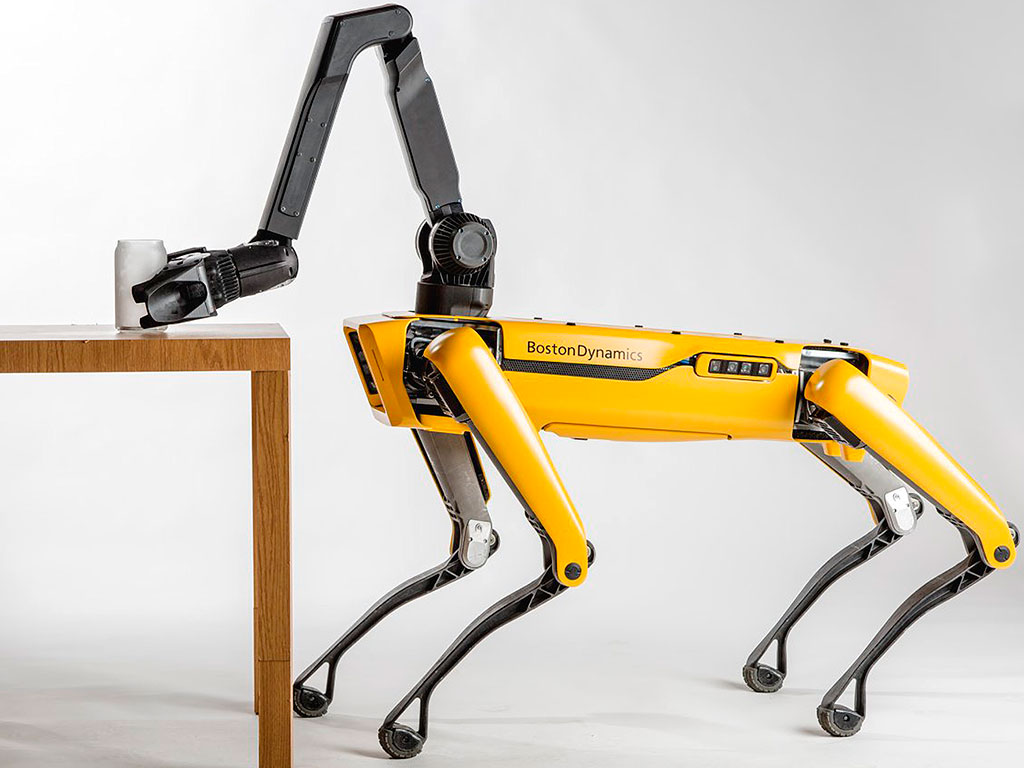
\includegraphics[keepaspectratio,width=0.8\textwidth]{assets/spotmini}
  \end{center}
\end{frame}

\begin{frame}{Learning to the Rescue?}
  There has been a lot of interest in learning for robot control and motion
  planning recently.

  \begin{center}
    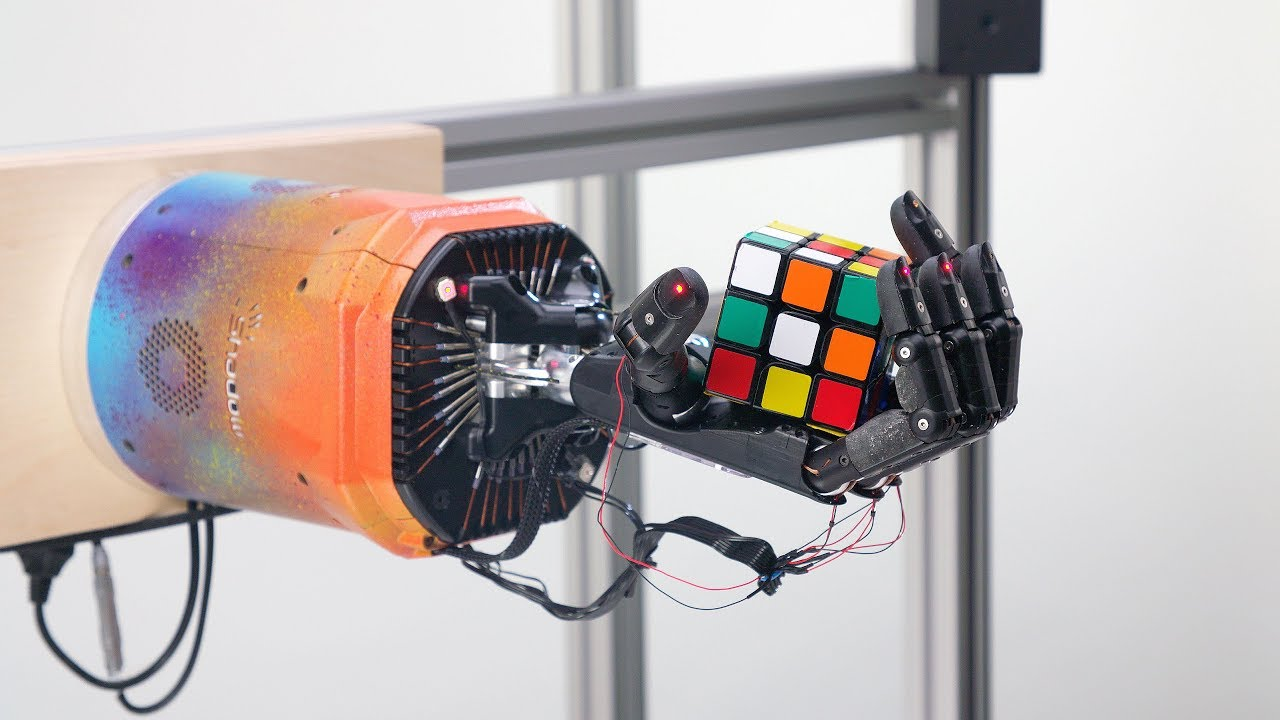
\includegraphics[keepaspectratio,width=\textwidth]{assets/openai_hand}
  \end{center}
\end{frame}

\begin{frame}{Big Data and Large Models}
  Deep learning leads us right back to expensive robots and questionable
  generalization. Where is learning taking place?

  \begin{center}
    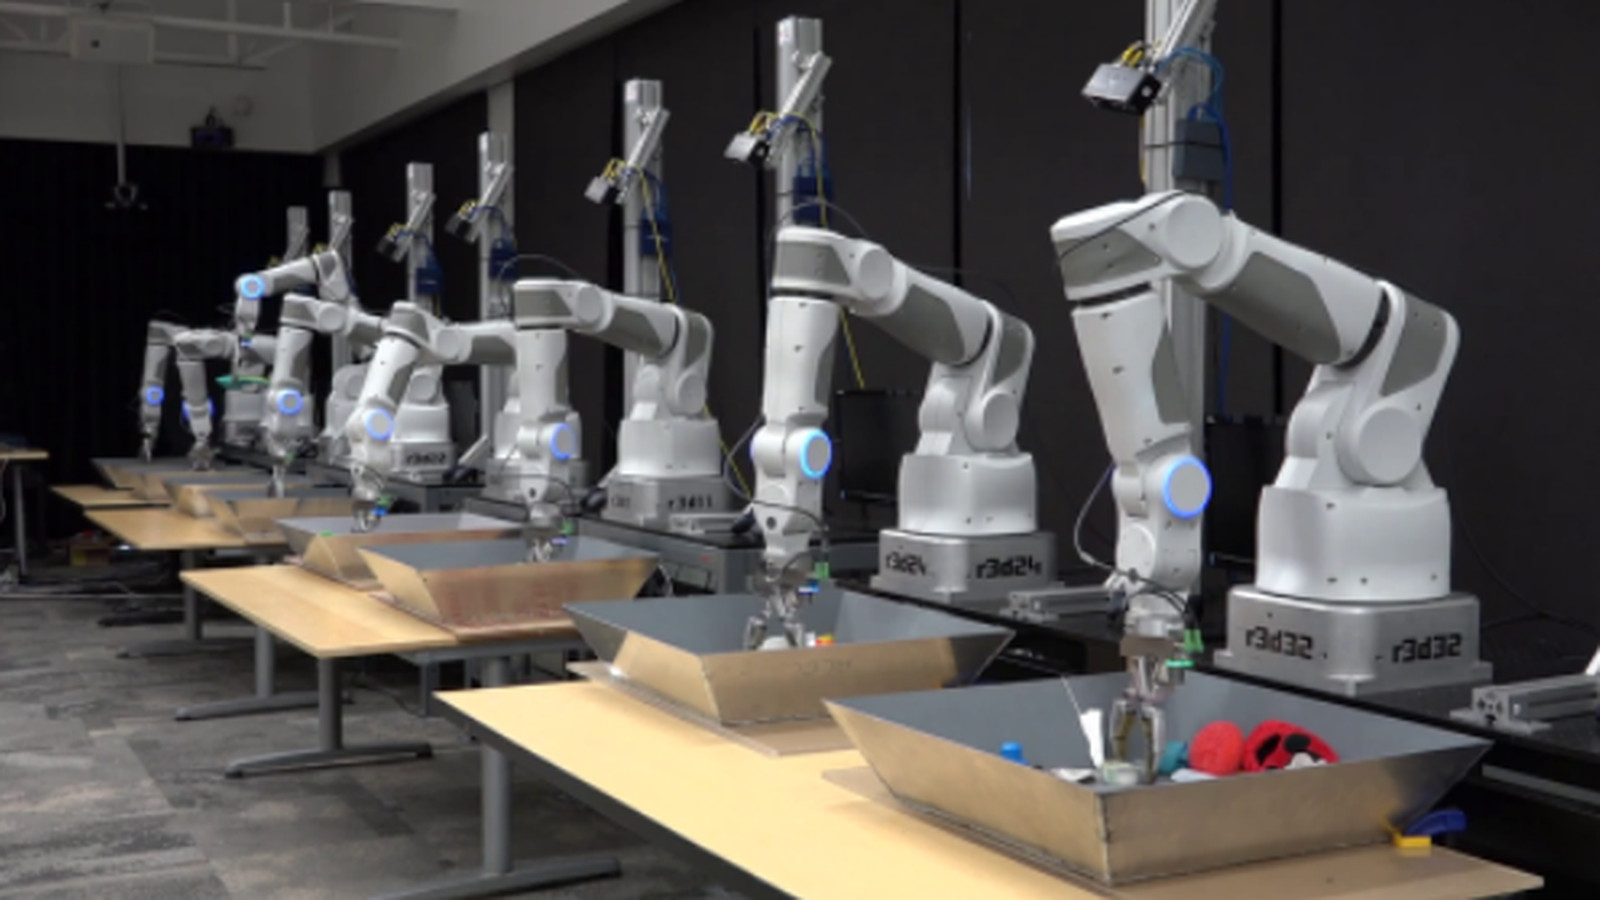
\includegraphics[keepaspectratio,width=0.8\textwidth]{assets/arm_farm}
  \end{center}
\end{frame}

\begin{frame}{How Safe Is Your Model?}
  \begin{itemize}
    \item Deep neural network controllers are not interpretable or verifiable
    \item Generalization is not well understood
    \item In any new situation, these controllers may be arbitrarily bad
  \end{itemize}
\end{frame}

\section{Reinforcement Learning}

\begin{frame}{RL Basics}
  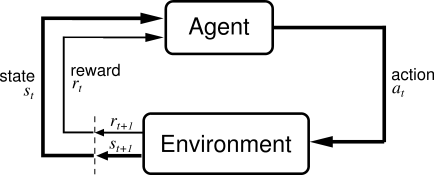
\includegraphics[keepaspectratio,width=\textwidth]{assets/agent_env}
\end{frame}

\begin{frame}{Notation}
  \begin{itemize}
    \item $x_t \in X$ (or $s_t$) are states, $u_t \in U$ (or $a_t$) are actions. 
    \item $r_t \in \mathbb{R}$ is a reward given by a \emph{reward function} $R : X \times U \rightarrow \mathbb{R}$.
    \item $P: X \times U \rightarrow X$ is a transition function.
    \item $\pi: X \rightarrow U$ is a \emph{policy} (or controller).
  \end{itemize}
\end{frame}

\begin{frame}{Value Functions}
  State value function\footfullcite{Sutton1998IntroductionTR}:
  \begin{equation}
    V_\pi(x) = \mathbb{E}\left[\sum_{t=0}^\top \gamma^t R(x_t, \pi(x_t)) \mid x_0 = x\right]
  \end{equation}
  satisfies Bellman equation
  \begin{equation}
    V_\pi(x) = \mathbb{E}\left[R(x, \pi(x)) + \gamma V_\pi(x_{t+1})\right]
  \end{equation}
\end{frame}

\begin{frame}{Policy Iteration}
  \begin{algorithm}[H]
      \DontPrintSemicolon
      \KwInput{An MDP $(X, U, R, P)$}
      \KwOutput{A policy $\pi$ optimizing rewards in the MDP}

      Initialize policy $\pi$ and $V_\pi$ \\
      \While {$\pi$ not stationary} {
        Estimate $V_\pi$ (\textbf{Policy Evaluation}) \\
        Set $\pi(x_t) = \argmax_{u_t} \left[r_t +  \gamma V_\pi(x_{t+1})\right]\ \forall x_t \in X$ \\ 
      }

      \textbf{Return} $\pi$

      \caption{Policy Iteration}
      \label{alg:stability_policy_iteration}
  \end{algorithm}
\end{frame}

\section{PARL in Three Parts}
\begin{frame}{Piecewise-Affine Reinforcement Learning}
  \scalebox{0.7} {
  \begin{algorithm}[H]
    \DontPrintSemicolon
    \SetAlgoLined
    \SetKwInOut{Input}{Input}
    \SetKwInOut{Output}{Output}
    \Input{A system to be controlled}
    \Output{A learned PARL controller}

    Sample reference points within state-space of $env$. \\
    Initialize $\hat{F}, \hat{V}$, and $\Pi$ to sensible defaults. \\
    \For{$i$ = $1\ldots training\_iterations$} {
      $data \leftarrow \emptyset$ \\
      \For{$j$ = $1\ldots num\_rollouts$} {
        $traj = do\_rollout(\Pi, env)$ \\
        $register\_experience(traj)$ \\
        $update\_dynamics(\hat{F})$ \\
        $update\_value\_function(\hat{V})$ \\
        $data \leftarrow data \cup traj$ \\
      }
      $update\_controller(\Pi, data)$ \\
      $data \leftarrow \emptyset$ \\
    }
    Return $\Pi$
    \caption{PARL}
  \end{algorithm}
  }
\end{frame}

\subsection{Partitioning}

\begin{frame}{What is a Partition?}
  We can loosely define a partition with indexing set $I$ of the state space $X$ as
  \begin{equation}
    P_I = \left\{\mathcal{V}_i \subseteq S\ \middle\vert 
      \begin{array}{l}
        i \in I, \\
        \bigcup_{i \in I}\mathcal{V}_i = S, \\
        \mathcal{V}_i \cap \mathcal{V}_j = \emptyset, \forall i \neq j
      \end{array}\right\}
  \end{equation}
\end{frame}

\begin{frame}{Implicit Voronoi Partition}
  Explicit polygonal partitions are expensive, so we define an implicit one by
  sampling \emph{reference points} and using a K-D Tree.\footfullcite{de1997computational}

  \begin{center}
    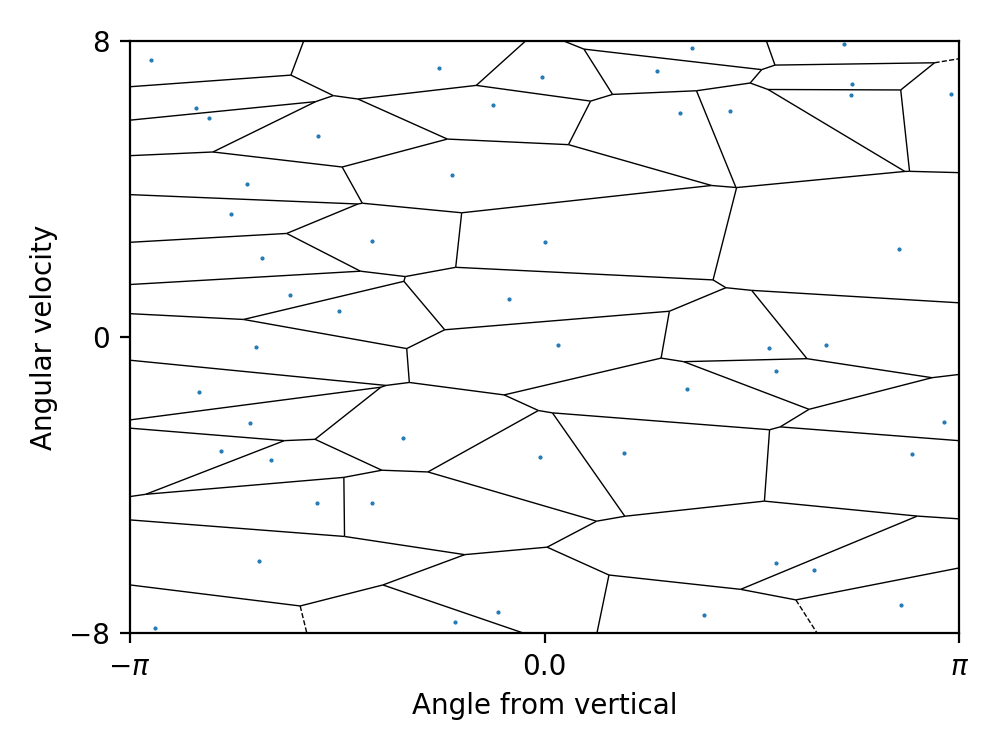
\includegraphics[keepaspectratio,width=0.7\textwidth]{assets/pendulum_voronoi}
  \end{center}
\end{frame}

\begin{frame}{Connections to Deep Neural Networks}
  Common deep neural network structures define implicit generalized Voronoi
  diagrams and piecewise-affine operators.\footfullcite{Balestriero2019TheGO} 

  \begin{center}
    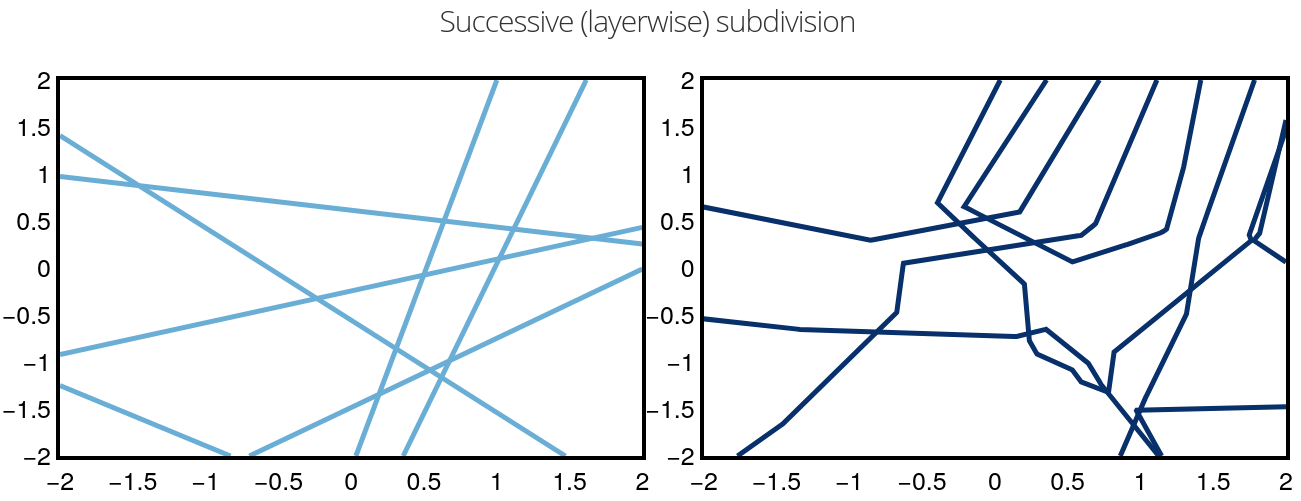
\includegraphics[keepaspectratio,width=0.8\textwidth]{assets/subdivision}
  \end{center}
\end{frame}

\subsection{Dynamics Estimation}

\begin{frame}{Local Linear Dynamics}
  We make a linear approximation to the local dynamics:
  \begin{equation}
    \hat{F}_{i}(\tilde{x}_t, u_t) = \hat{A}x_t + \hat{B}u_t + c 
  \end{equation}
  which can be estimated from data using \emph{Recursive Least Squares}
\end{frame}

\begin{frame}{Recursive Least Squares}
  The RLS filter is defined by
  \begin{align*}
    \phi_T &= \left[\begin{array}{l}x_t \\ u_t \end{array}\right] \\
    y_T &= x_{t+1}\\
    P_T &= P_{T-1} - \frac{P_{T-1}\phi_T \phi_T^\top P_{T-1}}{1 + \phi_T^\top P_{T-1} \phi_T} &\text{\emph{(Inverse sample covariance)}} \\
    \theta_T &= \theta_{T-1} + P_T \phi_T \left[y_T - \phi_T^\top \theta_{T-1} \right] &\text{\emph{(RLS parameter estimate)}}
  \end{align*}

  Note $\theta_T = \begin{bmatrix}\hat{A} \\ \hat{B}\end{bmatrix}$, and $\hat{c}$ can be estimated in a similar way.\footnote{See \url{http://cannontwo.com/assets/rls_notes.pdf}}
\end{frame}

\begin{frame}{Theoretical Guarantees}
  Assuming white noise corruption of the $y_T$ values, RLS converges almost
  surely to the true parameters. It can also be modified to deal with white
  noise corrupting $\phi_T$. However, $P_T$ must always have full rank.
\end{frame}

\begin{frame}{Practical Implementation}
  There are several implementation details:
  \begin{itemize}
    \item $P_0$ must be chosen arbitrarily
    \item Estimating $\hat{c}$ requires a little additional bookkeeping
    \item Forgetting factor $\lambda$ for time-varying parameters
  \end{itemize}
\end{frame}

\subsection{Value Function Approximation}

\begin{frame}{Local Value Function Approximation}
  Similar to the dynamics approximation, we make a linear approximation of the local dynamics:
  \begin{equation}
    \hat{V}^{\pi}_i(x_t) = V_0 + V_x^\top x_t
  \end{equation}
  which can be estimated using \emph{Least Squares Temporal Difference Learning}.
\end{frame}

\begin{frame}{Least Squares Temporal Difference Learning}
  The LSTD filter is a modified RLS filter, defined by:
  \begin{align*}
    \Delta &= \phi_T(x_t) - \gamma \phi_T(x_{t+1})\\
    C_{t+1} &= C_T - \frac{C_T \phi_T(x_t) \Delta^\top C_T}{1 + \Delta^\top C_t \phi_T(x_t)}\\
    d_{t+1} &= d_T + \phi_T(x_t)r_t
  \end{align*}
  and the corresponding parameters are given by $C_T d_T$, from which $V_0$ and $V_x$ can be extracted for each partition region.
\end{frame}

\begin{frame}{LSTD Theoretical Guarantees}
  LSTD has the same sort of theoretical results as the RLS filter, except that
  additional decorrelation conditions apply between $\Delta$ and $\phi_T(x_t)$.
\end{frame}

\begin{frame}{Practical Implementation}
  For PARL, we define
  \begin{align*}
    \phi_i(x_t) &= \begin{cases} \begin{bmatrix} x_t \\ 1 \end{bmatrix} & \text{for } x \in \mathcal{V}_i \\ 0  &\text{otherwise}\end{cases} \\
    \phi_T(x_t) &= \phi_i(x_t) \text{, stacked for all $i \in I$}
  \end{align*}
  This feature set defines a self-consistent piecewise-affine approximation to
  the value function on the PARL partition. However, it is computationally
  expensive to compute the LSTD approximation in this feature space. 
\end{frame}

\subsection{Controller Optimization}

\begin{frame}{Local Linear Controllers}
  We optimize a piecewise-affine controller in terms of local linear controllers defined by
  \begin{equation}
    \pi_i(x_t) = Kx_t + k
  \end{equation}
\end{frame}

\begin{frame}{Gradient-based Controller Updating}
  It is easy to compute empirical gradients of $V$ with respect to the local
  controller parameters $K$ and $k$ that apply at a state $x_t$:
  \begin{align}
    \nabla_K &= B^\top V_x x_t^\top \\
    \nabla_k &= B^\top V_x
  \end{align}
  Since we have a full estimate of the dynamics and value function, we can also
  do a line search rather than using a learning rate parameter. 
\end{frame}

\begin{frame}{Theoretical Guarantees?}
  \begin{itemize}
    \item There are not a lot of existing theoretical guarantees for empirical gradient controller updating
    \item However, the usage of a line search and consistent dynamics/value approximation may lead to guarantees
  \end{itemize}
\end{frame}

\subsection{Results}

\begin{frame}{The Inverted Pendulum}
  \begin{figure}
    \centering
    \begin{subfigure}{0.8\linewidth}
      \centering
      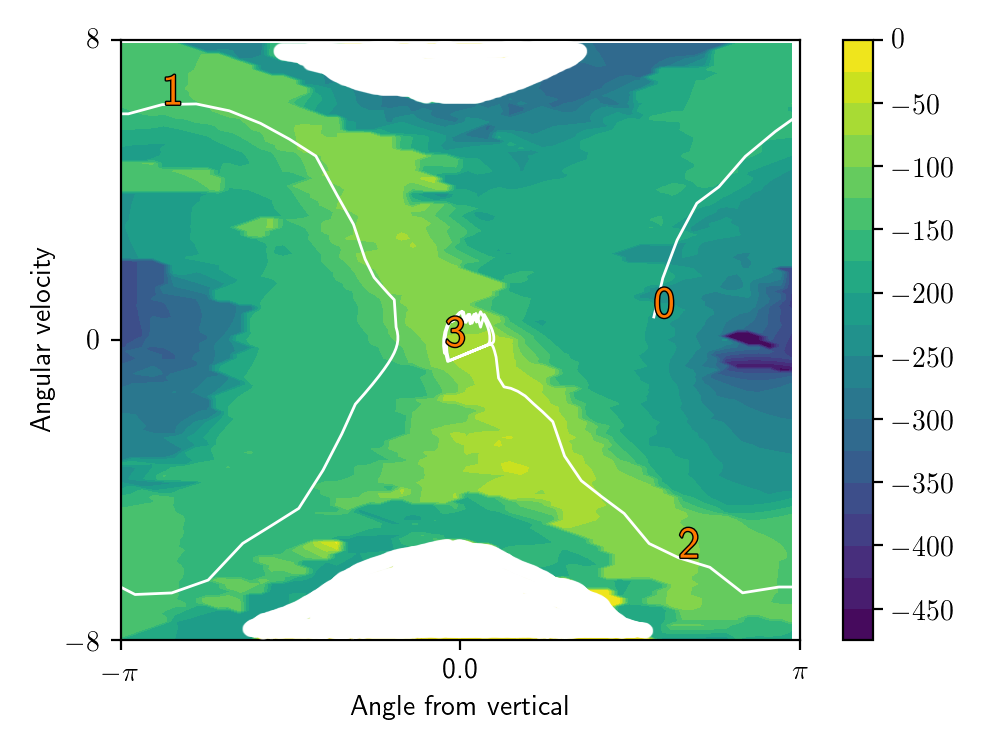
\includegraphics[width=\linewidth,trim=0 10 0 0,clip]{assets/pendulum_value}
      \vspace{-1em}
    \end{subfigure}
    \begin{subfigure}{0.2\linewidth}
      \centering
      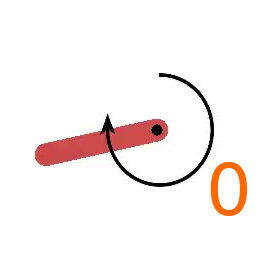
\includegraphics[width=\linewidth,trim=0 0 0 20]{assets/pendulum_traj_0}
    \end{subfigure}
    \begin{subfigure}{0.2\linewidth}
      \centering
      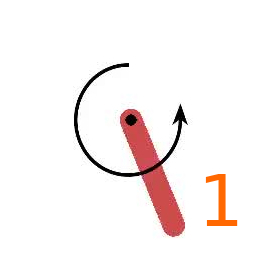
\includegraphics[width=\linewidth,trim=0 0 0 20]{assets/pendulum_traj_1}
    \end{subfigure}
    \begin{subfigure}{0.2\linewidth}
      \centering
      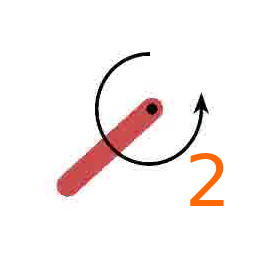
\includegraphics[width=\linewidth,trim=0 0 0 20]{assets/pendulum_traj_2}
    \end{subfigure}
    \begin{subfigure}{0.2\linewidth}
      \centering
      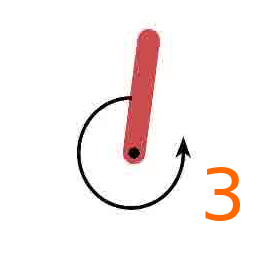
\includegraphics[width=\linewidth,trim=0 0 0 20]{assets/pendulum_traj_3}
    \end{subfigure}
  \end{figure}
\end{frame}

\begin{frame}{Reference Point Placement Experiments}
  \begin{figure}[htb]
      \centering
      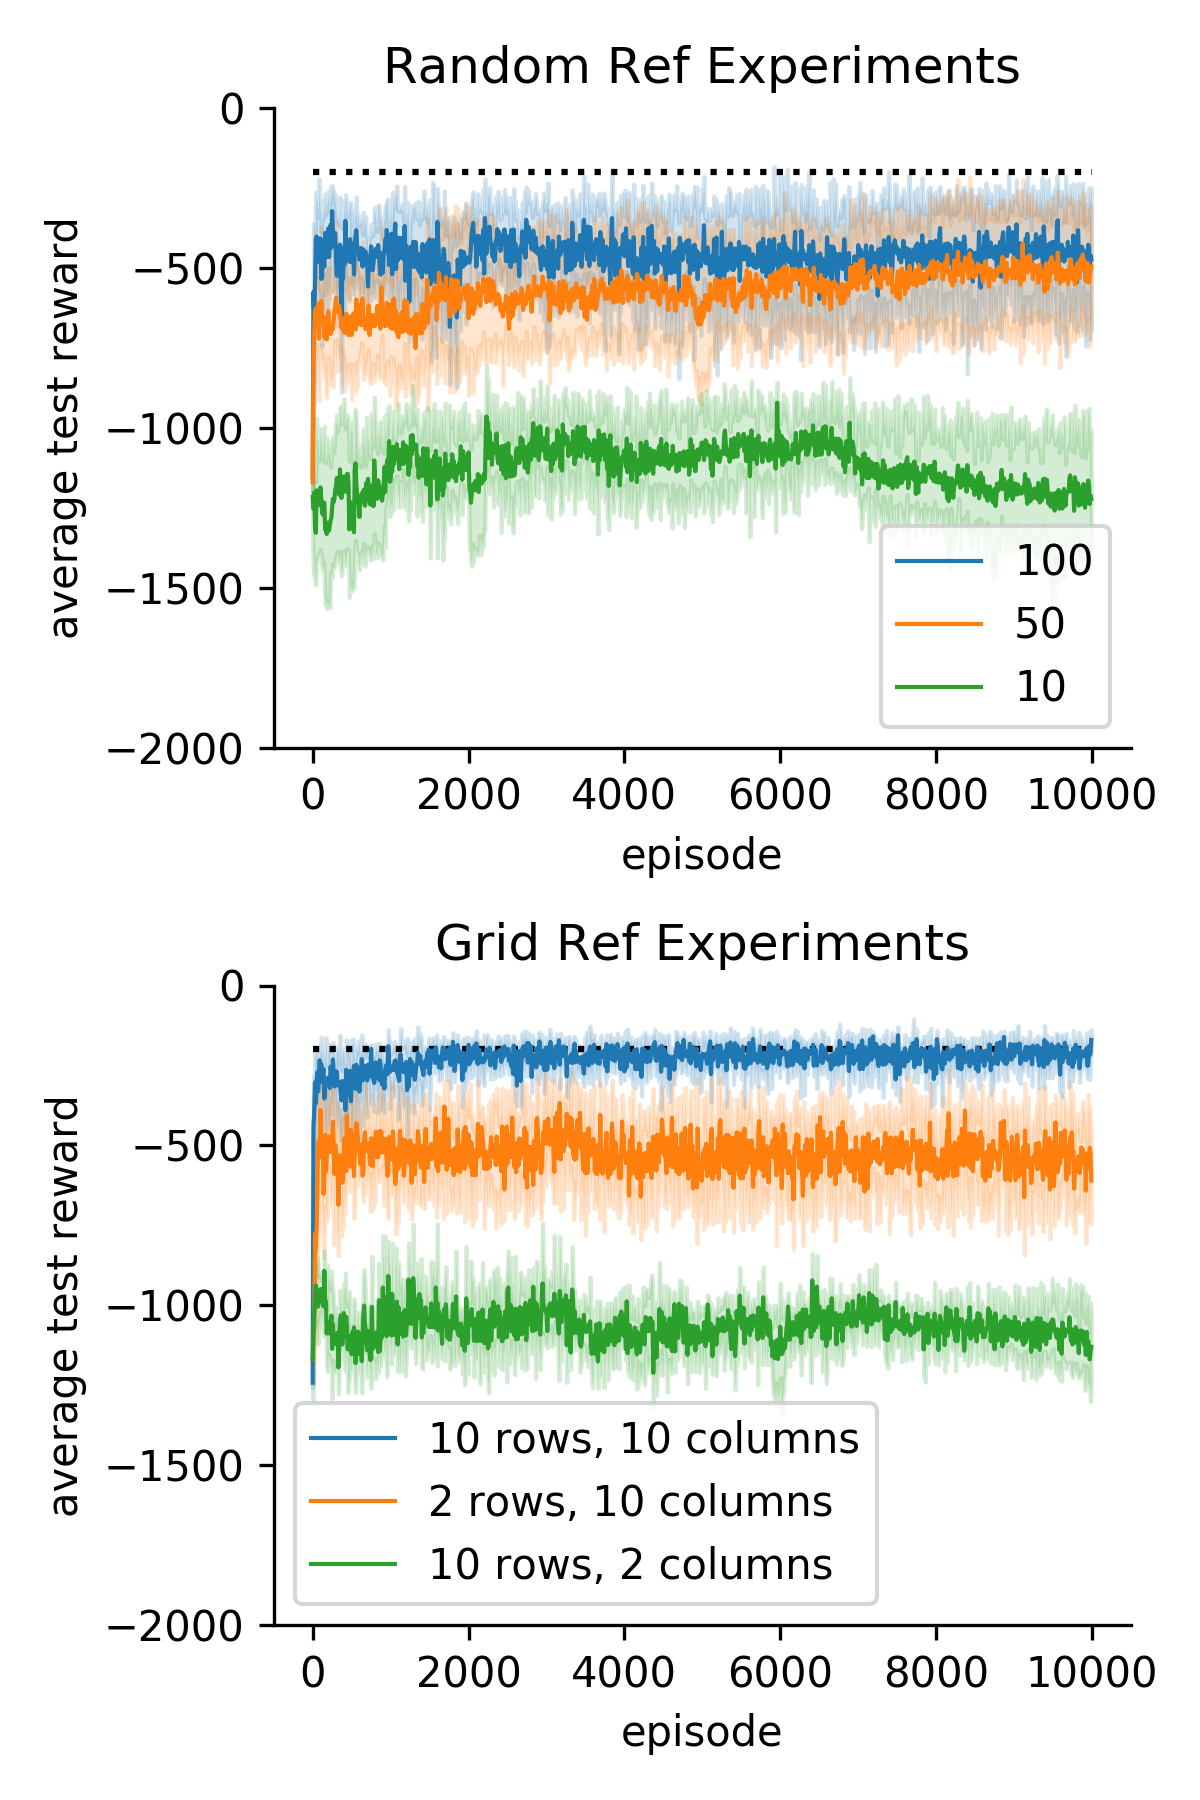
\includegraphics[width=0.5\linewidth,trim=0 0 0 0,clip]{assets/combined_ref_exps}
  \end{figure}
\end{frame}

\begin{frame}{Interpretability Experiments: Value Functions}
  \begin{figure}[t]
    \centering
    \begin{subfigure}{0.30\linewidth}
      \centering
      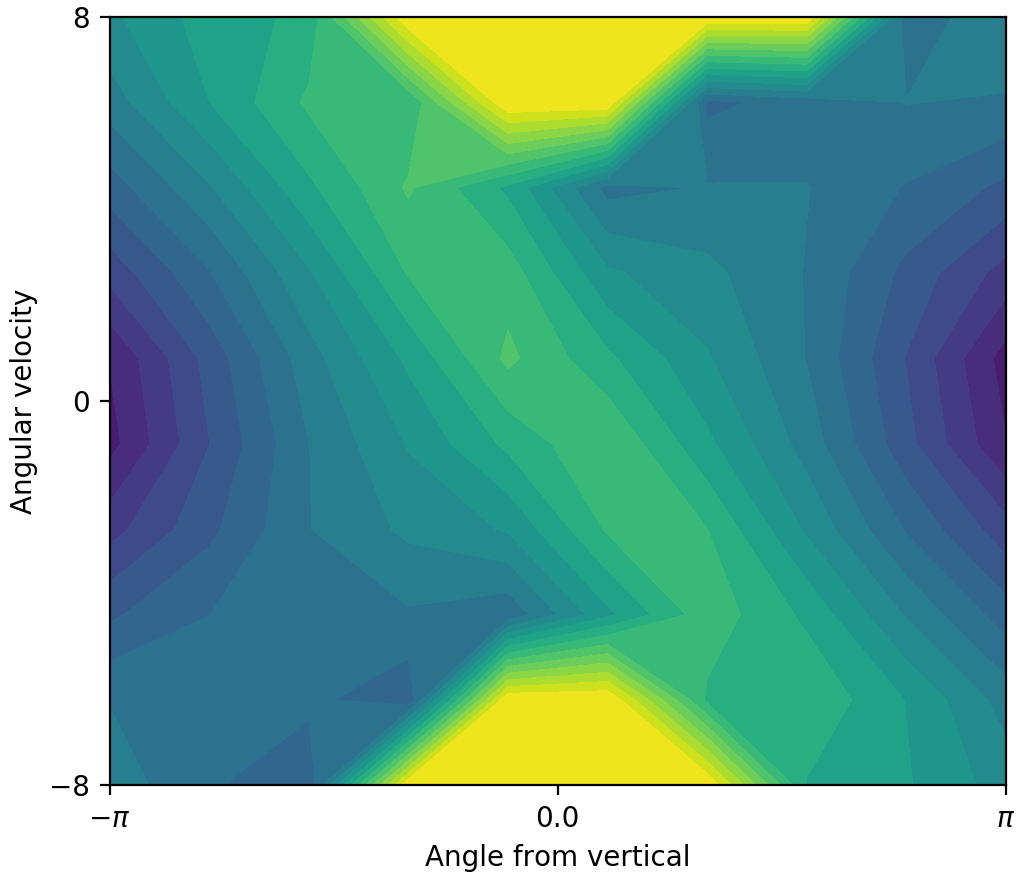
\includegraphics[width=0.9\linewidth,trim=0 0 0 0,clip]{assets/ref_plots/value_model_refcolexps_r10c10_1_ep0}
      \caption{0 episodes}
    \end{subfigure}
    \begin{subfigure}{0.30\linewidth}
      \centering
      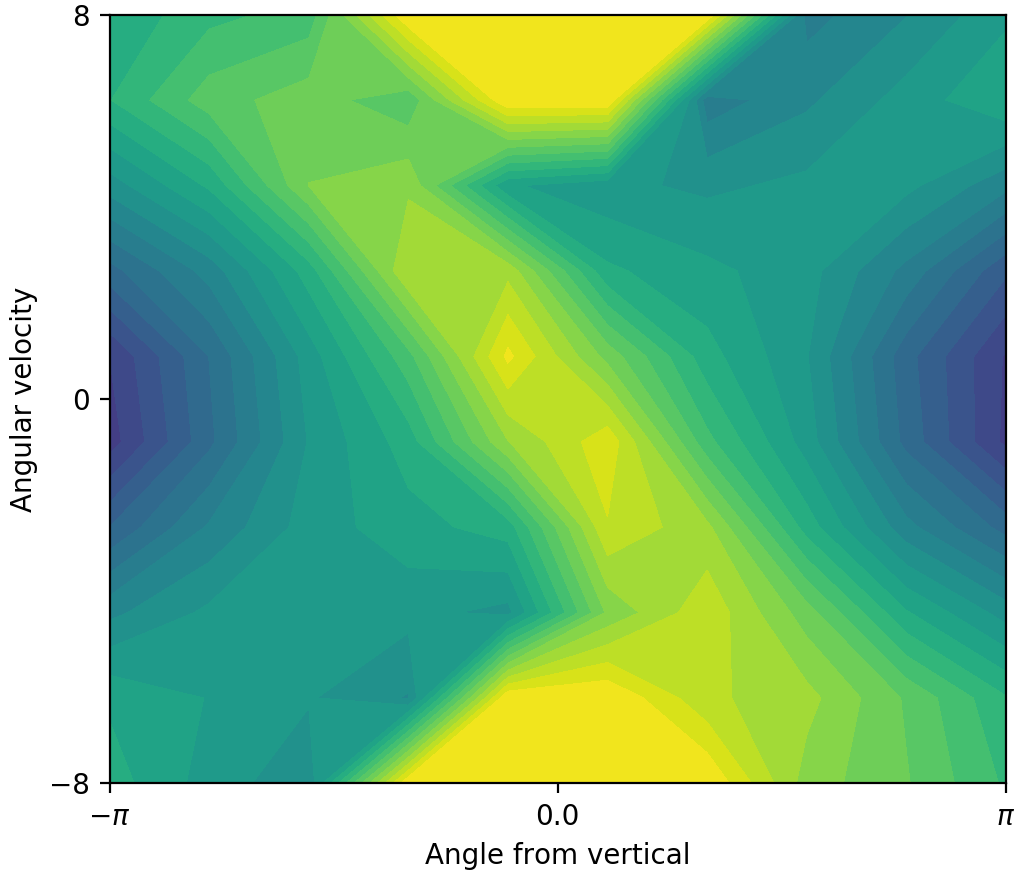
\includegraphics[width=0.9\linewidth,trim=0 0 0 0,clip]{assets/ref_plots/value_model_refcolexps_r10c10_1_ep1000}
      \caption{1000 episodes}
    \end{subfigure}
    \begin{subfigure}{0.30\linewidth}
      \centering
      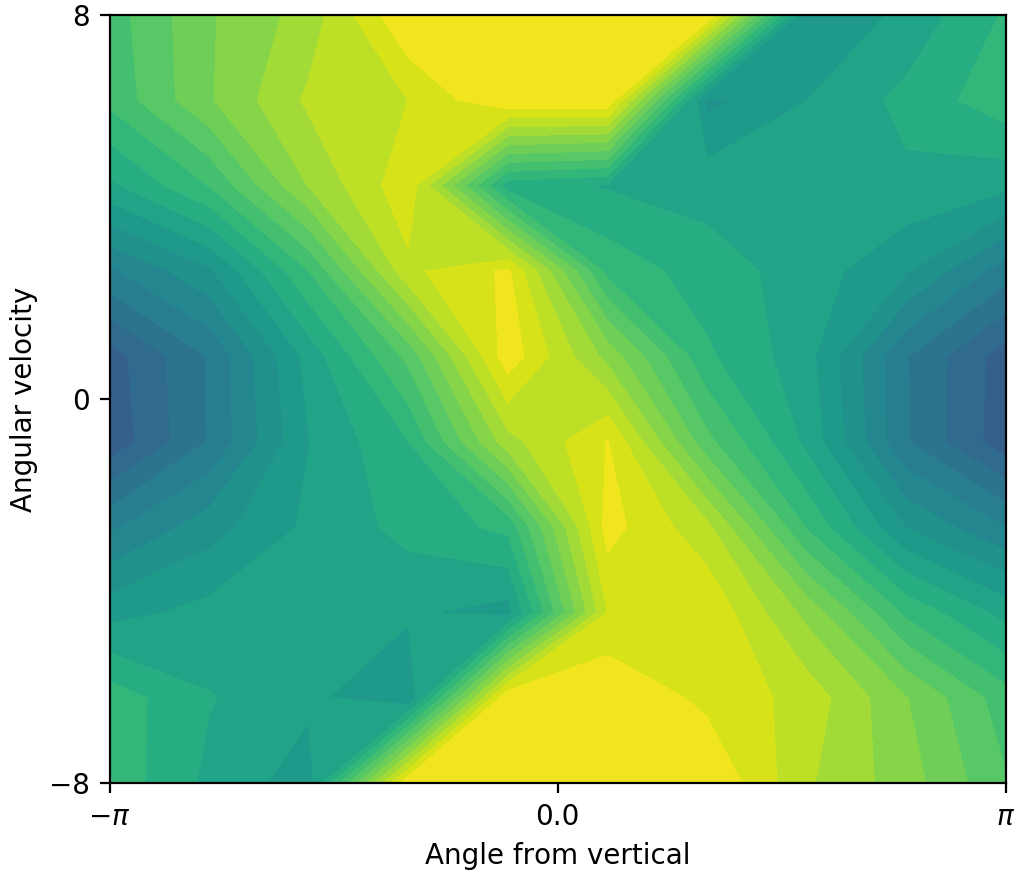
\includegraphics[width=0.9\linewidth,trim=0 0 0 0,clip]{assets/ref_plots/value_model_refcolexps_r10c10_1_ep9900}
      \caption{9900 episodes}
    \end{subfigure}
    \begin{subfigure}{0.05\linewidth}
      \vspace{-2em}
      \centering
      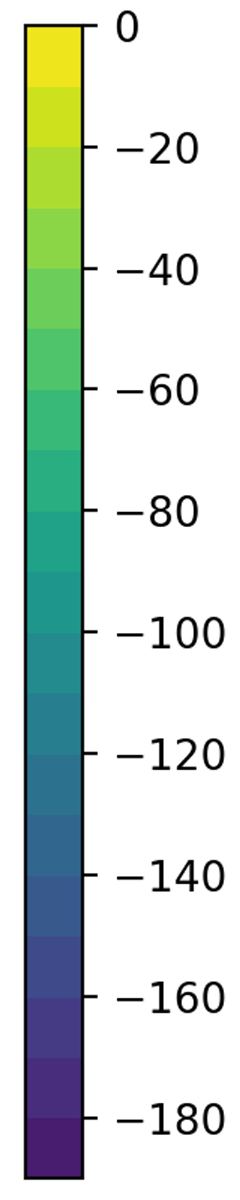
\includegraphics[width=\linewidth,trim=0 0 0 0,clip]{assets/ref_plots/r10c10_colorbar}
    \end{subfigure}
    \begin{subfigure}{0.30\linewidth}
      \centering
      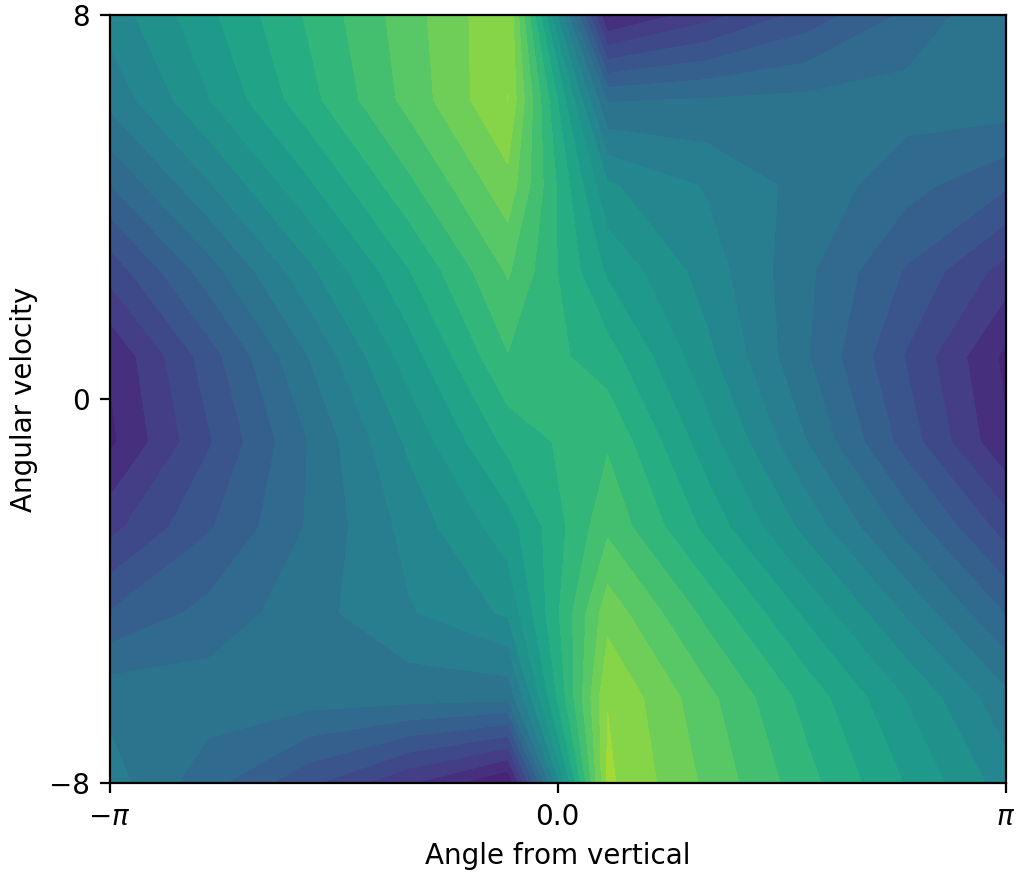
\includegraphics[width=0.9\linewidth,trim=0 0 0 0,clip]{assets/ref_plots/value_model_refcolexps_r10c2_1_ep0}
      \caption{0 episodes}
    \end{subfigure}
    \begin{subfigure}{0.30\linewidth}
      \centering
      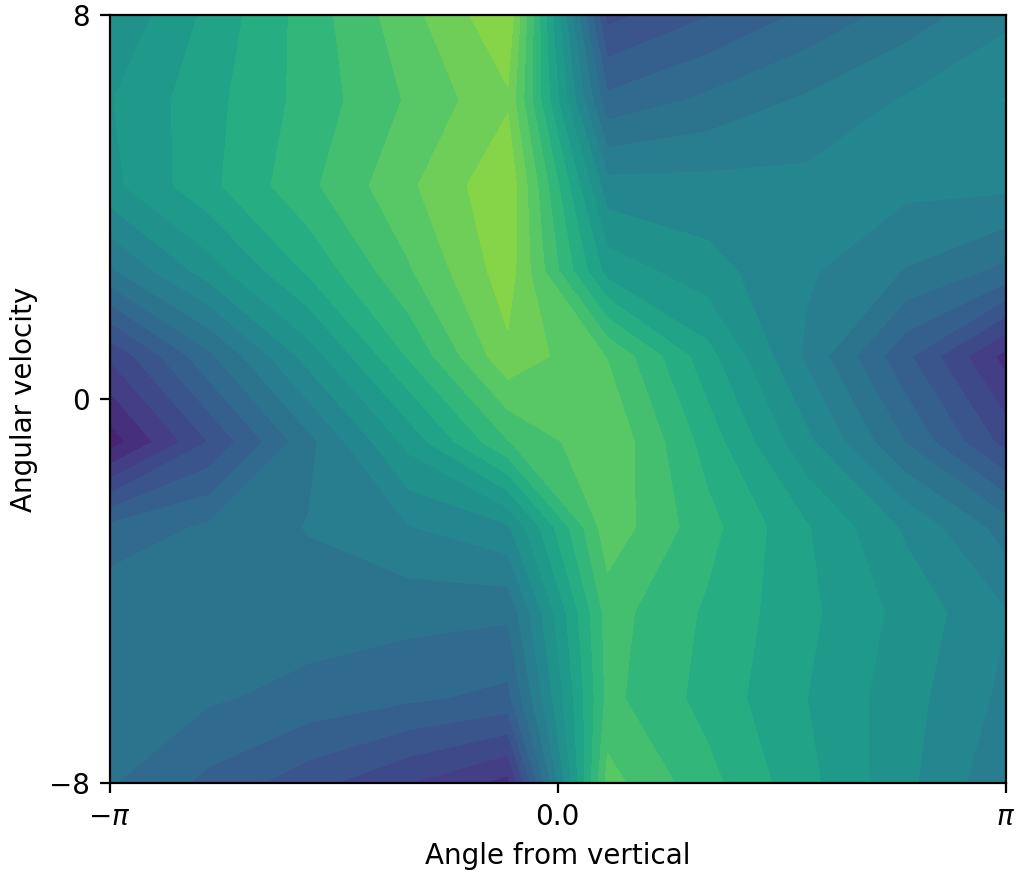
\includegraphics[width=0.9\linewidth,trim=0 0 0 0,clip]{assets/ref_plots/value_model_refcolexps_r10c2_1_ep1000}
      \caption{1000 episodes}
    \end{subfigure}
    \begin{subfigure}{0.30\linewidth}
      \centering
      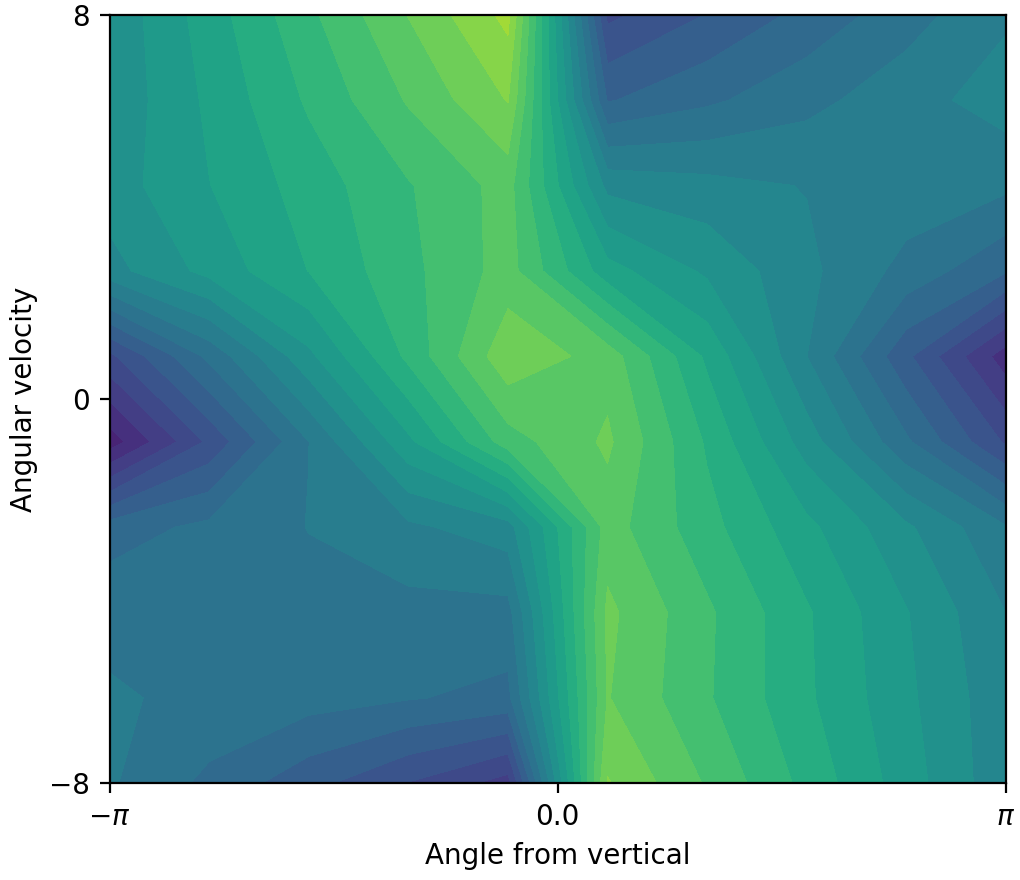
\includegraphics[width=0.9\linewidth,trim=0 0 0 0,clip]{assets/ref_plots/value_model_refcolexps_r10c2_1_ep9900}
      \caption{9900 episodes}
    \end{subfigure}
    \begin{subfigure}{0.05\linewidth}
      \vspace{-2em}
      \centering
      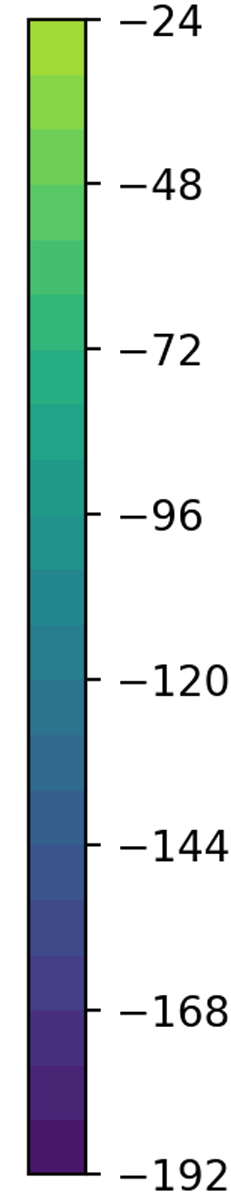
\includegraphics[width=\linewidth,trim=0 0 0 0,clip]{assets/ref_plots/r10c2_colorbar}
    \end{subfigure}
    \caption{Value functions computed by PARL over the course of training. Top Row: 10 rows/10 columns of reference points. Bottom Row: 10 rows/2 columns of reference points. }
  \end{figure}
\end{frame}

\begin{frame}{Interpretability Experiments: Controllers}
  \begin{figure}[t]
    \centering
    \begin{subfigure}{0.30\linewidth}
      \centering
      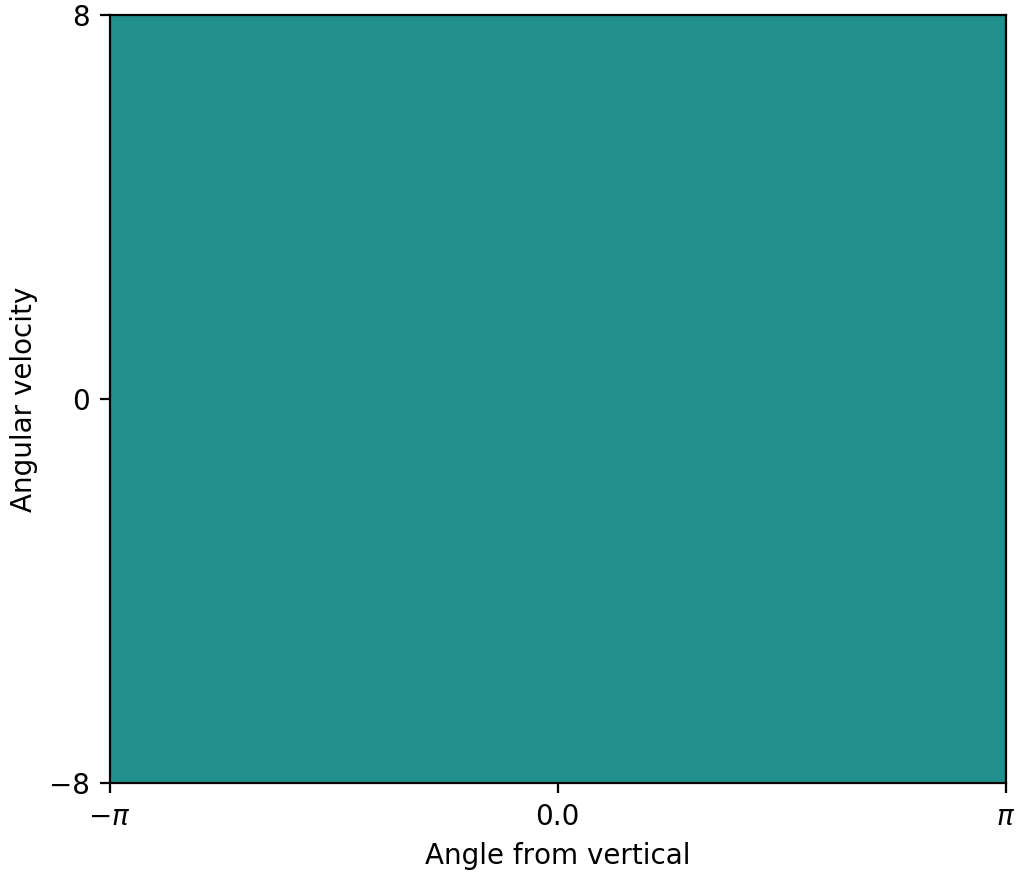
\includegraphics[width=0.9\linewidth,trim=0 0 0 0,clip]{assets/ref_plots/controller_refcolexps_r10c10_1_ep0}
      \caption{0 episodes}
    \end{subfigure}
    \begin{subfigure}{0.30\linewidth}
      \centering
      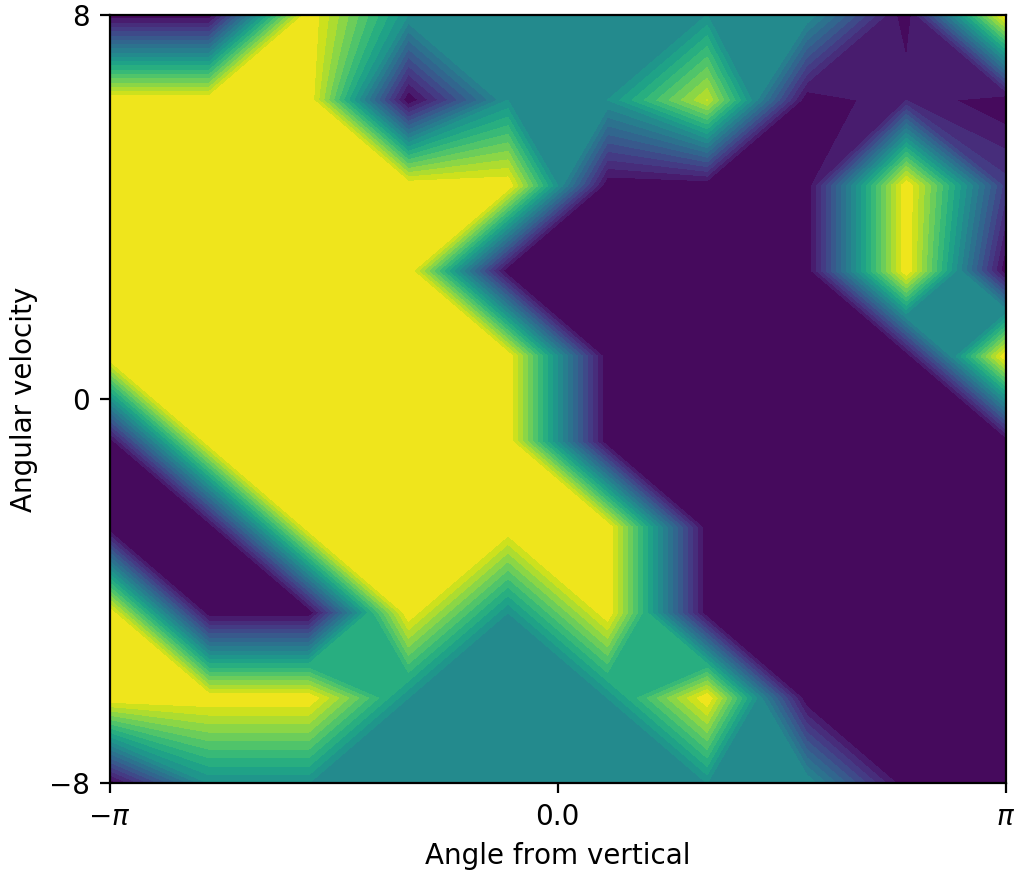
\includegraphics[width=0.9\linewidth,trim=0 0 0 0,clip]{assets/ref_plots/controller_refcolexps_r10c10_1_ep1000}
      \caption{1000 episodes}
    \end{subfigure}
    \begin{subfigure}{0.30\linewidth}
      \centering
      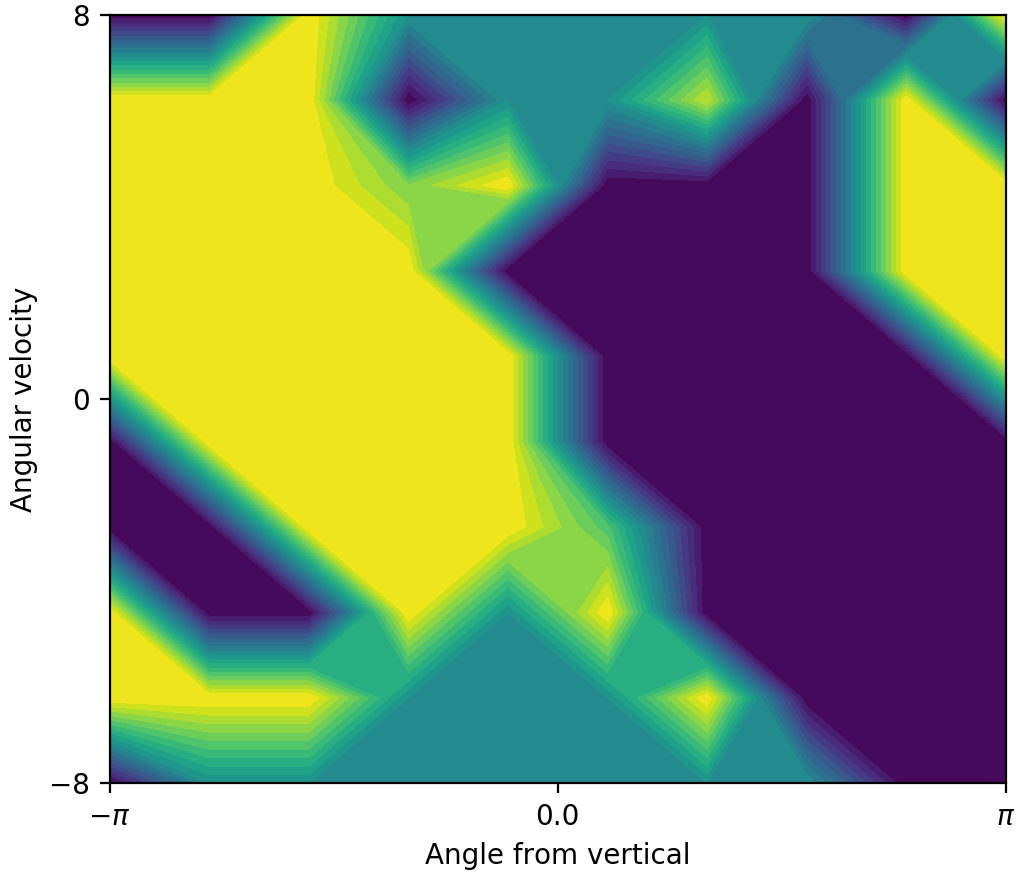
\includegraphics[width=0.9\linewidth,trim=0 0 0 0,clip]{assets/ref_plots/controller_refcolexps_r10c10_1_ep9900}
      \caption{9900 episodes}
    \end{subfigure}
    \begin{subfigure}{0.05\linewidth}
      \vspace{-2em}
      \centering
      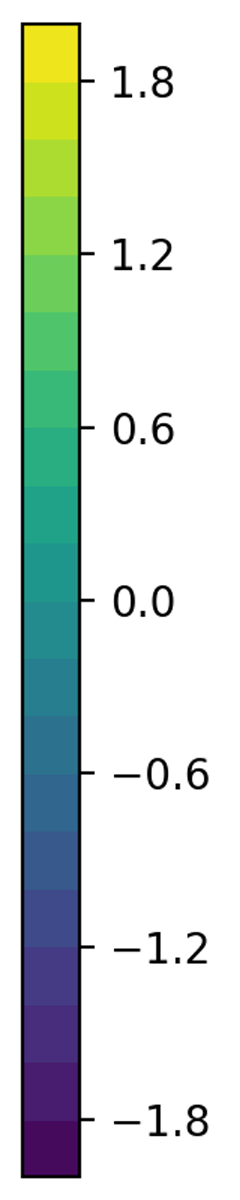
\includegraphics[width=\linewidth,trim=0 0 0 0,clip]{assets/ref_plots/controller_colorbar}
    \end{subfigure}
    \begin{subfigure}{0.30\linewidth}
      \centering
      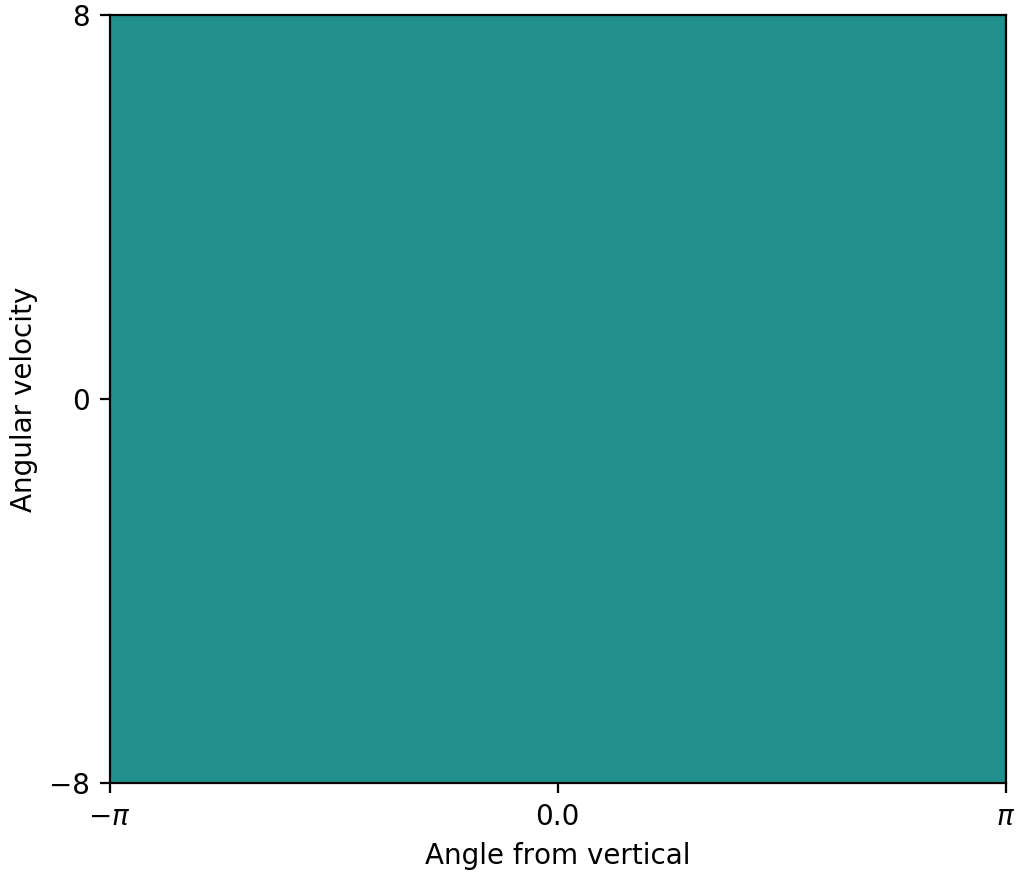
\includegraphics[width=0.9\linewidth,trim=0 0 0 0,clip]{assets/ref_plots/controller_refcolexps_r10c2_1_ep0}
      \caption{0 episodes}
    \end{subfigure}
    \begin{subfigure}{0.30\linewidth}
      \centering
      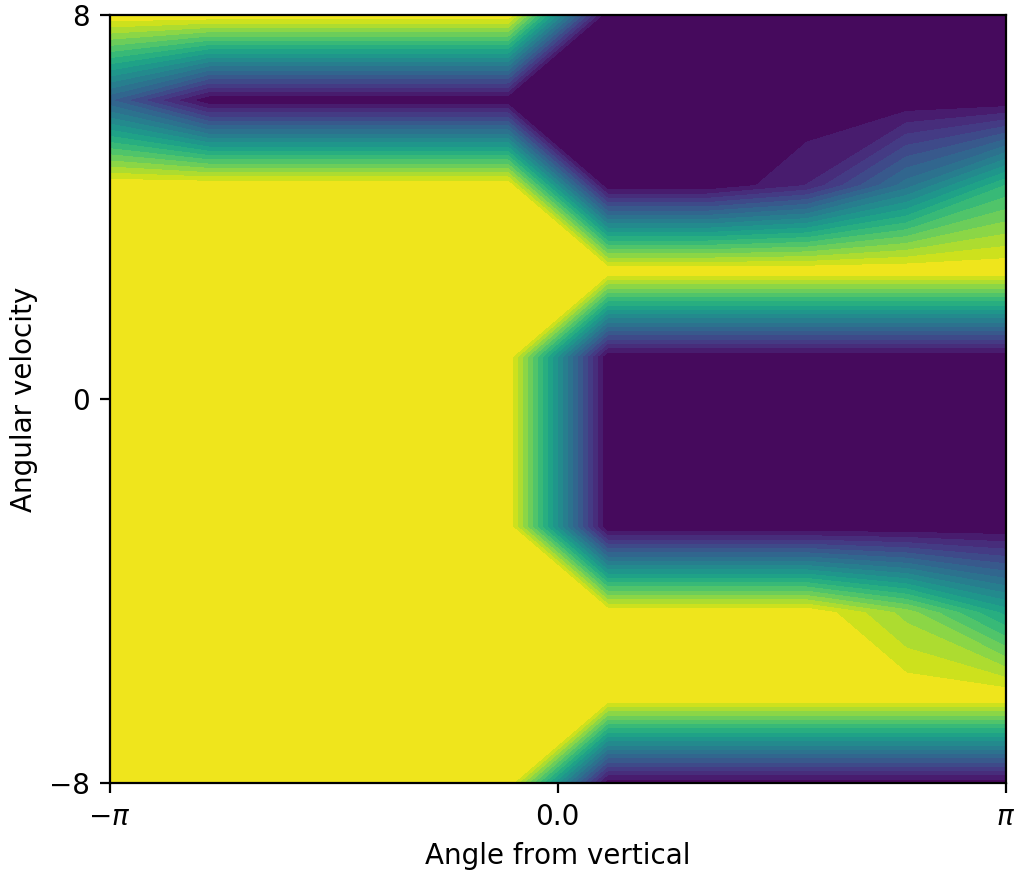
\includegraphics[width=0.9\linewidth,trim=0 0 0 0,clip]{assets/ref_plots/controller_refcolexps_r10c2_1_ep1000}
      \caption{1000 episodes}
    \end{subfigure}
    \begin{subfigure}{0.30\linewidth}
      \centering
      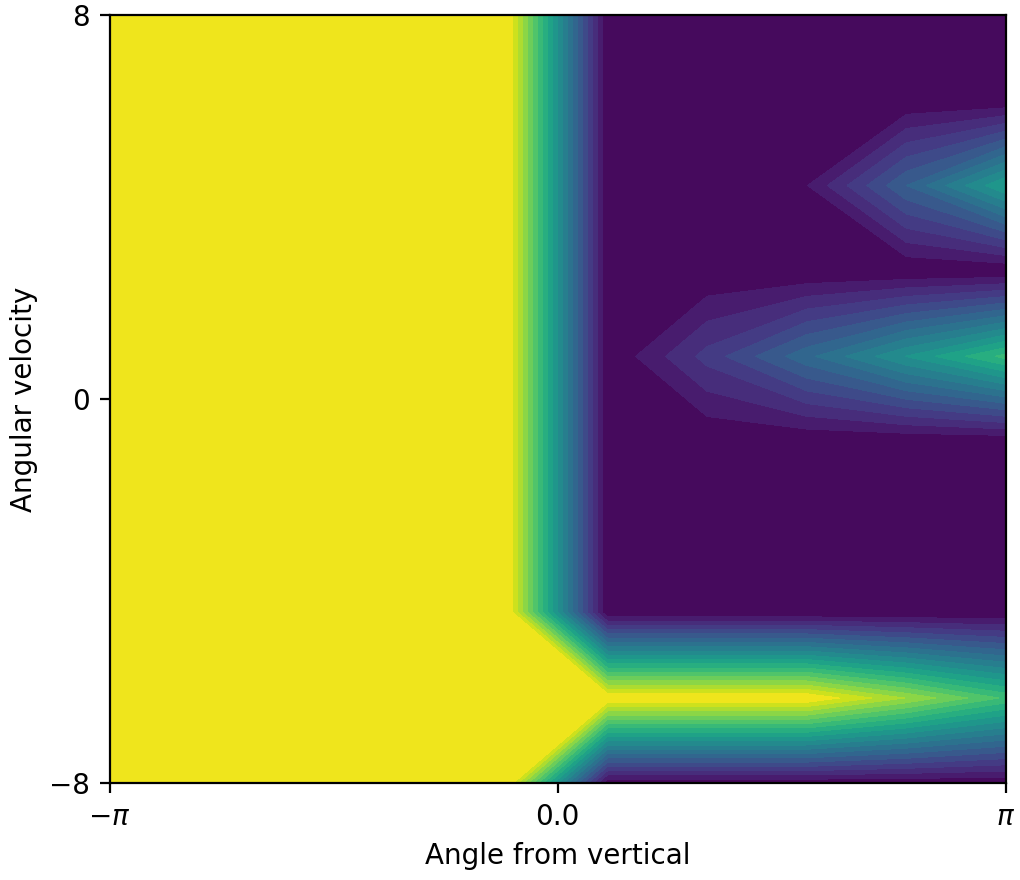
\includegraphics[width=0.9\linewidth,trim=0 0 0 0,clip]{assets/ref_plots/controller_refcolexps_r10c2_1_ep9900}
      \caption{9900 episodes}
    \end{subfigure}
    \begin{subfigure}{0.05\linewidth}
      \vspace{-2em}
      \centering
      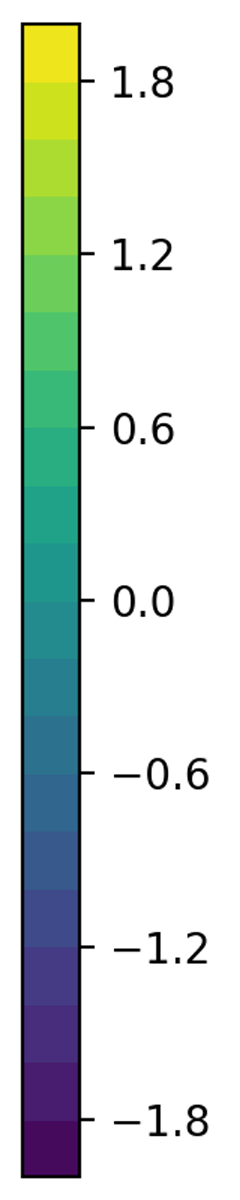
\includegraphics[width=\linewidth,trim=0 0 0 0,clip]{assets/ref_plots/controller_colorbar}
    \end{subfigure}
    \caption{Controllers learned by PARL over the course of training. Top Row: 10 rows/10 columns of reference points. Bottom Row: 10 rows/2 columns of reference points.}
  \end{figure}
\end{frame}


\section{Stability of PARL Controllers}

\begin{frame}{Stability in Control}
  Given a state $\bar{x}$ that we want to stabilize around, how do we design
  controllers which drive the state of the system to $\bar{x}$, even in the
  presence of disturbances?

  Using PARL, we can approximately solve this problem by using the reward function
  \begin{equation*}
    R(x, u) = ||x - \bar{x}||
  \end{equation*}
\end{frame}

\begin{frame}{Lyapunov Functions}
  In discrete time, a \emph{Lyapunov function}\footfullcite{khalil2002nonlinear} $V: X \rightarrow \mathbb{R}$ is a function such that
  \begin{align}
    V(x) \geq 0 \text{ } \forall x \in X \\
    V(\bar{x}) = 0  \\
    V(x_{t+1}) - V(x_t) \leq 0
  \end{align}
  Such functions can be used to prove stability of a system around $\bar{x}$.
\end{frame}

\begin{frame}{Kinds of Stability}
  In addition to basic Lyapunov stability, we have
  \begin{itemize}
    \item \emph{Asymptotic stability}: $V(x_{t+1}) - V(x) < 0$, and so the system monotonically proceeds to $\bar{x}$.
    \item \emph{Exponential stability}: If $V(x)$ decreases faster than an exponential function of $x$, and so the system proceeds ``quickly'' to $\bar{x}$.
  \end{itemize}
  For this stability exploration, we only consider basic Lyapunov stability.
\end{frame}

\begin{frame}{Piecewise-Affine Lyapunov Functions}
  In order to find piecewise-affine Lyapunov functions for the PARL-controlled
  system, we solve a linear program in terms of the partition, piecewise-affine
  dynamics estimate, and piecewise-affine controller. This LP comes from Rubagotti et al.\footfullcite{Rubagotti2012StabilityAO}
\end{frame}

\begin{frame}{Mesh Refinement}
  \begin{algorithm}[H]
      \DontPrintSemicolon
      \KwInput{PWA controller system, maximum number of iterations}
      \KwOutput{Estimate of the region of attraction $P$ and Lyapunov certificate of ES($P$)}
      
      \For{$i < $ maximum iterations}{
          \If{$i > 1$}{
              $\mathcal{X}_i = \mathcal{X}_{ij}, \Omega_{ip}$ \\
              $\mathcal{X} = \bigcup \mathcal{X}_i$
          }    
          Compute the sets $\mathcal{X}_{ij}$ and $\Omega_{ip}$ \\
          Attempt to solve the LP \\
          \If{the LP has a solution}{
              Estimate the region of attraction $P$ \\
              \textbf{Return} the LP solution and $P$
          }
      }
      
      \textbf{Return} $P$ undefined

      \caption{Stability Analysis}
      \label{alg:stability_lp}
  \end{algorithm}
\end{frame}

\begin{frame}{Inverted Pendulum Results}
  \begin{figure}[t]
      \centering
      
      \begin{subfigure}{0.9\linewidth}
          \centering
          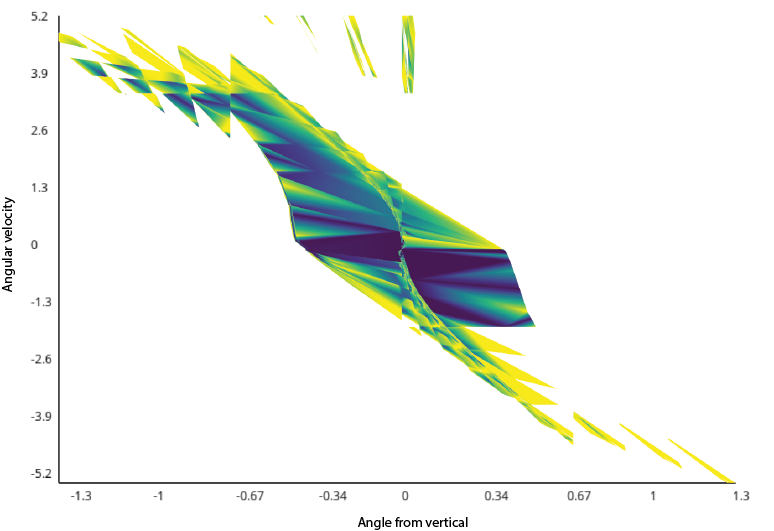
\includegraphics[width=0.95\linewidth,trim=0 0 0 0,clip]{assets/lyapunov}
      \end{subfigure}
      \begin{subfigure}{0.08\linewidth}
          \centering
          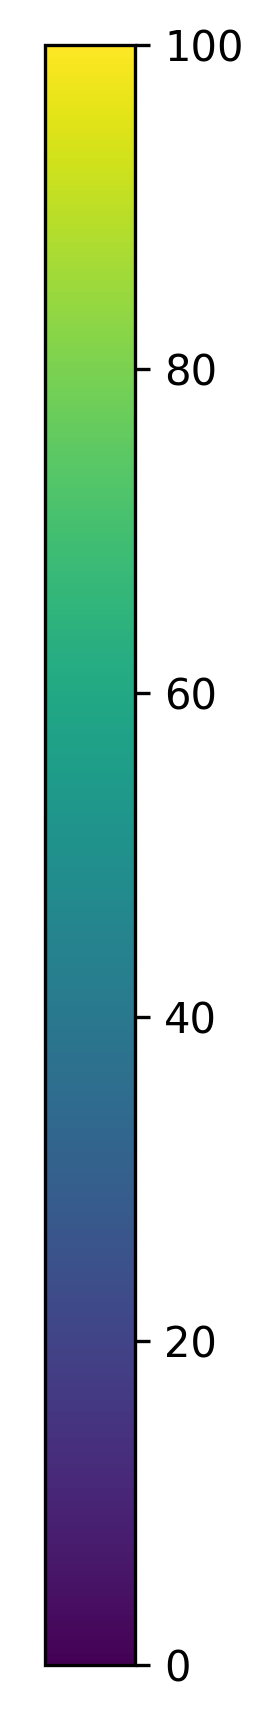
\includegraphics[width=\linewidth,trim=0 0 0 0,clip]{assets/viridis_lyap.png}
      \end{subfigure}
  \end{figure}
\end{frame}

\section{Future Work}

\begin{frame}{There's a lot}
  \begin{enumerate}
    \item PARL+Planning
    \item Theoretical Results
    \item Adaptive Partitioning
    \item Integrating Uncertainty
  \end{enumerate}
\end{frame}

\subsection{PARL+Planning}

\begin{frame}{Nominal Models}
  In most robotics applications, we have access to some kind of nominal model.
  It's not reasonable to throw that model away when we want to do learning.
\end{frame}

\begin{frame}{Learning Errors}
  Suppose that the real system is of the form
  \begin{equation*}
    x_{t+1} = F(x_t) + G(x_t)u_t
  \end{equation*}
  and we are given a nominal model of the form 
  \begin{equation*}
    \bar{x}_{t+1} = \bar{F}(x_t) + \bar{G}(x_t)u_t
  \end{equation*}
  Then we want to estimate $\hat{F}, \hat{G}$ such that 
  \begin{align*}
    x_{t+1} &\approx \bar{x}_{t+1} + \hat{F}(x_t) + \hat{G}(x_t)u_t \\
    &\approx \left(\bar{F} + \hat{F}\right)(x_t) + \left(\bar{G} + \hat{G}\right)(x_t)u_t
  \end{align*}
\end{frame}

\begin{frame}{Tracking Control and Model Updating}
  We want to estimate these error dynamics with PARL, while simultaneously
  using PARL to do learned trajectory-tracking control.

  \begin{center}
  \scalebox{0.7} {
    \begin{algorithm}[H]
      \DontPrintSemicolon
      \KwInput{Nominal model $model$,\\ 
      \quad Execution environment $env$,\\ 
      \quad Planner $planner$,\\
      \quad a deviation parameter $\epsilon$,\\
      \quad $start$, $goal$}
      
      \SetKwFunction{ExecutePath}{ExecutePath}
      \SetKwFunction{UpdateModel}{UpdateModel}
      \SetKwFunction{Plan}{Plan}

      \BlankLine
      $planning\_model \leftarrow$ Aggregate nominal \& learned model, initialized by $model$ \\
      \While{Not at goal} {
          $p \leftarrow$ \Plan{$planner$, $planning\_model$, $start$, $goal$, $obstacles$} \\
          $PARL \leftarrow$ PARL agent for use error state space around $p$ \\
          
          \ExecutePath{$env$, $p$, $PARL$, $\epsilon$}
          
          $start \leftarrow$ current state of $env$ \\
          \UpdateModel{$planning\_model$, $PARL$, $p$}
      }
      \caption{PARL + Planning}
      \label{alg:parl_planning}
  \end{algorithm}
  }
  \end{center}
\end{frame}

\subsection{Theoretical Results}

\begin{frame}{PARL Algorithmic Stability}
  Establishing the stability of learned controllers is nice, but we also want
  guarantees about the PARL algorithm itself. Under what conditions does it
  converge to a near-optimal controller? 
\end{frame}

\begin{frame}{PARL Algorithmic Robustness}
  What effect does environment stochasticity have on the PARL algorithm? How
  can the learning algorithm be made robust to various forms of noise and
  uncertainty?
\end{frame}

\subsection{Adaptive Partitioning}

\begin{frame}{Extension to Varying Mesh}
  One of the biggest criticisms of PARL is that its performance depends on
  reference point placement. This raises the following questions:
  \begin{itemize}
    \item Can reference points be sampled from experienced data? (similar to a Gaussian Process)
    \item Can reference points be adjusted during learning?
    \item How does varying the mesh during learning affect stability and robustness?
  \end{itemize}
\end{frame}

\begin{frame}{Adaptation Strategies}
  Several strategies for adjusting the partition during learning are possible:
  \begin{itemize}
    \item Lloyd's algorithm\footfullcite{Kanungo2002AnEK}
    \item Splitting/Merging in response to uncertainty
    \item Hinging Hyperplanes\footfullcite{Sjberg1995NonlinearBM}
  \end{itemize}
\end{frame}

\subsection{Explicit Uncertainty}

\begin{frame}{Sources of Uncertainty}
  RLS and LSTD provide measures of sample uncertainty in the form of inverse
  sample covariance matrices. These can be incorporated into the controller
  update step in order to make the PARL algorithm more robust. Uncertainty may
  also be key to making PARL+Planning work.
\end{frame}

\begin{frame}{Other Forms of Uncertainty}
  We could conceive of a Bayesian PARL which makes use of priors over the
  dynamics and controller in order to be even more robust. 

  \begin{itemize}
    \item What form should these priors take? 
    \item How would else would the algorithm need to change?
    \item Are the theoretical guarantees for PARL strengthened?
    \item Can the algorithm still be made efficient?
  \end{itemize}
\end{frame}

\section{Questions?}

\end{document}
